\chapter{Software and Computing}
\label{ch:detectors-sc}

\subsection{Overview}

The scope of the Software and Computing effort includes the design \fixme{and what else, coding, 
purchasing resources, coordinating effort ??}. The principal areas of focus are the computing 
infrastructure, the far detector physics software and the near detector physics software. \fixme{no section for ND yet}.

The requirements for the Software and Computing are given throughout this chapter according to the expected data rates \fixme{}


\section{Computing Infrastructure}
\label{sec:detectors-sc-infrastructure}

\fixme{I moved this up to introduce the section}
The computing infrastructure for DUNE is designed to handle data streams present in
oscillation physics studies with beam neutrinos, since these data will constitute the bulk of what is 
committed to mass storage, transmitted over networks, processed offline and, in general, impose the 
most significant infrastructure and cost considerations. Issues and parameters related to other classes of 
data are covered in \anxrates, as well as in Section~\ref{sec:detectors-fd-ref-daq}. \fixme{`` and other 
sections.'' If there are other sections, let's identify them, maybe in the fd alt chap and nd chap?} This 
annex contains information on both the Reference Design and Alternate Design versions of the Far Detector.
%\subsection{Single Phase Design and the Alternate design} -- sectioning not needed for this. Anne
However, the bulk of this section describes characteristics of data in the context of the single-phase LAr detector. 
Implications of the alternate design (see Section~\ref{sec:detectors-fd-ref-ov}) are outlined in 
Section~\ref{sec:detectors-sc-alternate}.

The DUNE Detector Systems that will be discussed are:
\begin{itemize}
\item Far Detector LAr TPC, Photon Detector(PD)
\item Near Detector (ND) Straw Tracker (STT), Calorimeter(CAL), Muon Detector Resistive Plate Chambers (RPC)
\end{itemize}


%\subsubsection{Assumptions} <--- moved up and `unsectioned'
%\label{sec:detectors-sc-infrastructure-assumptions}

%According to the present baseline design, the Far Detector (Liquid Argon TPC) in 


%the issue of possible variations in the design and/or characteristics between these modules shall not be addressed, as there is no concrete information developed at this point to support this approach. 
A few basic assumptions will be used: \fixme{These are not raw-data-specific; I think they're assumptions for designing the computer infrastructure, no? That's why I moved them up}
\begin{itemize}
\item The DUNE far detector will consist of four %identical  
modules of \tpcdetectormass each.
\item For purposes of this document the detector modules are taken to be identical.
\item %Estimates presented below correspond to 
The detector mass is the sum of the four modules, i.e., %,  is effectively normalized to 
\dunedetectormass.
\item The accelerator spill cycle is \beamspillcycle.
\item Zero-suppression thresholds will be set at levels that preserve signals from minimum-ionizing particles.
\item The intensity of the beam provided by LBNF will affect the data rates for a few detector
systems in DUNE (cf. the Near Detecor). \fixme{can we be specific? Won't the beam affect data rates in both detectors?}
\item The beam characteristics are taken as documented in \vollbnf.
\item The front-end systems of the TPC and the Photon Detector, combined
with the logic in DAQ, will provide triggering capability for the beam neutrino physics; 
triggering outside of the beam spills will be provided by the DAQ utilizing continuously digitized
data from the photon detection system. %light readout system.
\end{itemize}



\subsection{Discussion of Physics Processes and Raw Data Rates} 

\label{sec:detectors-sc-infrastructure-data-rates}
% -- taken care of (anne)-- \fixme{A special Annex document for data rates was updated on 4/23/2015. It covers most DUNE physics and background processes but the information is still being examined and modified. It is the reference document on which important paramaters of the DUNE data are based.The Annex contains information on both the Reference Design and Alternate Design versions of the Far Detector.}

%\subsubsection{Classes of Raw Data} % you used `class' rather than `type' above


%DUNE is a multipurpose apparatus and the variety of physics goals to be pursued during its operation will be reflected in different characteristics of respective data streams processed and collected in real time and offline.
DUNE is a multipurpose apparatus designed to pursue a variety of physics objectives. It will thus
require multiple data streams with differing characteristics that will be processed and collected in both real time and offline. \fixme{Is this right?}
%
%As one example, consider the difference between neutrino oscillations physics done with beam neutrinos on one hand, and the ambitious goal of detecting the rare Supernova bursts (SNB) on the other.
For example, signals produced by beam events will be characterized by total energy in the GeV range, allowing
%appropriate
 thresholds for zero-suppression (ZS) to be set at the levels appropriate for
minimum-ionizing particles, %which 
greatly reducing the
background component of the data. Beam-based data will rely mostly on offline processing. By comparison, the energy scale of the signals produced by
SNB neutrino interactions %in the active volume of the detector 
is estimated to be in the range of tens
of MeV, %resulting in 
requiring much lower thresholds to be set for this type of measurement, and therefore
a considerable (if not overwhelming) rate of SNB-specific data coming
out of the LArTPC in real time, with contribution from radiological backgrounds.
Another differentiating SNB feature is that \textit{multiple neutrinos are expected
to arrive and interact in the detector volume} %during the possible rare Supernova burst event 
within seconds
of each other. %, as opposed to a single vertex produced by a beam neutrino (or any other localized interactions and/or decays).
To support the SNB physics, a massive sample of data from multiple low-energy
depositions will need to be processed ``on the fly''
using approaches and algorithms that are completely  different from those for the
beam neutrino physics. %, which mostly relies on offline processing. (moved up)

\subsection{Estimated Data Rates} % New section title from Anne

In the following, estimated data rates for %these components 
the detector systems are itemized and then aggregated. Certain parameters may be rounded off where appropriate. % I moved this last sentence here (anne)

%There will be cases where no reliable estimates exist at the moment due to continued R\&D, and this will
%be clearly stated where necessary.
It will be noted wherever reliable estimates are not yet available.  

\subsubsection{Far Detector LArTPC}
The rates presented in this section are derived from
the parameters listed in \anxrates. %Consider the following LAr TPC parameters:
\begin{itemize}
\item TPC channel count: \dunenumberchannels (i.e., four times
  \daqchannelsperdetector, which is the channel count for each \tpcdetectormass module)
\item Maximum drift Time: \tpcdrifttime
\item Number of drift time windows in one DAQ readout cycle: \daqdriftsperreadout
\item ADC clock frequency: approx. \daqsamplerate
\item ADC resolution (bits): 12
\end{itemize}
\
The following are factors affecting data rates and volumes:
\begin{itemize}
\item Zero Suppression (ZS)  in the front-end electronics of the detector
\item Radiological and Cosmological Backgrounds as functions of thresholds set for ZS
and DAQ trigger configuration (cf. the case of low-energy events)
\end{itemize}

Non-ZS maximum event size (corresponding to a snapshot of the complete TPC) can be calculated as a product of the following numbers:
\begin{itemize}
\item Channel count
\item Number of ADC samples per total drift (collection) time
\item Drift time windows in one DAQ cycle
\item ADC resolution
\end{itemize}
\
This results in a total of \dunefsreadoutsize worth of TPC data in one
readout.
The effect of zero suppression on
the beam-neutrino event size is dramatic, and Monte Carlo studies done with realistic neutrino
energy spectra suggest that it will be $\sim$\beameventsize.
However, %one of the possibilities that is
%now actively explored by 
the DUNE DAQ team is actively exploring the possibility of
recording beam event candidates (e.g., events with signals
above the ``high threshold'' as detailed in the Annex) at very low or no threshold, corresponding
to a virtually full data stream.
In this case, one can estimate the annual total %size of the 
TPC data collection
%to be collected annually 
by multiplying the predicted number of beam-neutrino interactions
per year (estimated here to be \beamrate) by the full uncompressed event size quoted above (\dunefsreadoutsize), yielding
%Thus one arrives to 
an annual estimate of \beamdatayearfs. % for each year of this type of data.

Some of the driving zero-suppressed (ZS) and full-scale (FS) annual
data volumes are summarized in Table~\ref{tab:sc-zs-summary}.
\fixme{The $^{39}$Ar data rate is probably not correct as depending on
  the ZS level much of its spectrum is below threshold.
This still needs further work from physics and DAQ groups.}
\begin{table}[htbp]
  \centering
  \caption{Annual data volume estimations for zero-suppressed (ZS) data from various sources.
  An additional full-stream (FS) data estimation is given for supernova burst (SNB).}
  % do not edit, this is generated by dune-params

\begin{cdrtable}[Annual data volume estimations for zero-suppressed (ZS) data from various sources.]{rrrrr}{sc-zs-summary}{Annual data volume estimations for zero-suppressed (ZS) data from various sources. An additional full-stream (FS) data estimation is given for supernova burst (SNB).}
Source & Event Rate & Event Size & Data Rate & Annual Data Volume \\ \toprowrule
$^{39}Ar$ (ZS) & \SI[round-mode=places,round-precision=1]{11.16}{\mega\hertz} & \SI[round-mode=places,round-precision=0]{150.0}{\byte} & \SI[round-mode=places,round-precision=1]{1.674}{\giga\byte\per\second} &  \SI[round-mode=places,round-precision=0]{52.8262940816}{\peta\byte}\\
all in-spill & & & & \SI[round-mode=places,round-precision=0]{158.558121686}{\tera\byte} \\
with-beam-$\nu$ & & & & \SI[round-mode=places,round-precision=0]{79.279060843}{\giga\byte} \\
\colhline
cosmic-$\mu$ (ZS) & \SI[round-mode=places,round-precision=3]{0.258947264}{\hertz} &
\SI[round-mode=places,round-precision=1]{2.5}{\mega\byte} & \SI[round-mode=places,round-precision=1]{647.36816}{\kilo\byte\per\second} &
\SI[round-mode=places,round-precision=0]{20.4289491035}{\tera\byte} \\
\colhline
beam-$\nu$ (ZS) & \SI[round-mode=places,round-precision=0]{8770.19567714}{\per\year} & \SI[round-mode=places,round-precision=1]{2.5}{\mega\byte} &
\SI[round-mode=places,round-precision=2]{0.694791666667}{\kilo\byte\per\second} & \SI[round-mode=places,round-precision=0]{21.9254891928}{\giga\byte} \\
beam-$\nu$ (FS) & \SI[round-mode=places,round-precision=0]{8770.19567714}{\per\year} & \SI[round-mode=places,round-precision=1]{24.8832}{\giga\byte} &
\SI[round-mode=places,round-precision=0]{6.915456}{\mega\byte\per\second} & \SI[round-mode=places,round-precision=0]{218.230533073}{\tera\byte} \\
\colhline
SNB cand. (ZS) & \SI[round-mode=places,round-precision=0]{12.0}{\per\year} & \SI[round-mode=places,round-precision=1]{16.74}{\giga\byte} &
\SI[round-mode=places,round-precision=0]{6365.63904105}{\byte\per\second} & \SI[round-mode=places,round-precision=0]{200.88}{\giga\byte} \\
SNB cand. (FS) & \SI[round-mode=places,round-precision=0]{12.0}{\per\year} & \SI[round-mode=places,round-precision=1]{46.08}{\tera\byte} &
\SI[round-mode=places,round-precision=1]{17.5226192958}{\mega\byte\per\second} & \SI[round-mode=places,round-precision=0]{552.96}{\tera\byte} \\
\end{cdrtable}
  \label{tab:sc-zs-summary}
\end{table}
\fixme{Can you put the generated table into cdrtable format?} 

\subsubsection{Far Detector Photon Detector (PD)}
There are variations in the basic parameters of the Photon Detector currently in the R\&D stage, %so
and the numbers in this section %presented below need to be considered as ballpark values to be 
will made more precise
at a later time:

\begin{itemize}
\item Readout channel count: 24,000 (i.e., four times 6,000 per 10-kt module)
\item Trigger rate not yet certain; %is uncertain at this point due to ongoing investigation; 
one possible approach assumes 1 trigger per spill cycle
\item ADC resolution (bits): 12
\end{itemize}
\
This results in 36~kB per spill cycle, and should be considered negligible % from the point of view of requirement to data handling, 
compared to other data sources.

\subsubsection{Near Detector Data Rates}
%Once again, t
The Near Detector is subject to an intense R\&D effort and its
parameters are still being optimized.% and not fixed at this point. 
The most relevant parameters
of the Fine-Grained Tracker (FGT) are:
\begin{itemize}
\item   Straw Tube Tracker (STT) readout channel count: 215,040
\item STT Drift Time: 120~ns
\item STT ADC clock frequency and resolution (bits): 3-ns intervals, 10~bit
\item ECAL channel count: 52,224
\item Muon Detector Resistive Plane Chambers (RPC) channel count: 165,888
\item Average expected event rate per spill: $\sim$1.5
\end{itemize}
\
Based on these parameters, the upper limit of the ND data rate can be estimated as 1.5~MB/s. This translates into $\sim$45~TB/year. 

\subsection{Processed Data}
\label{sec:detectors-sc-infrastructure-processed-data}
For the purposes of this document, processed data %is defined as 
includes most data which is not considered ``raw,'' i.e., data derived from raw (including possibly multiple stages
of calibration and reconstruction) as well as data produced from Monte Carlo studies.

The amount of expected processed data is still uncertain, however, 
%There are uncertainties in anticipated quantities of all of these types of data.
depending on the optimum readout strategy, an annual raw data volume of
\SI{1}{\tera\byte} to \SI{1}{\peta\byte} %may be collected.
is estimated. 
%Assuming that the data will undergo a few 
Given the processing stages, one can expect % the need
to handle as much as $\sim$\SI{2}{\peta\byte} of data annually for reconstruction and a lesser
volume for final analysis. % purposes.

At the time of writing. typical annual volume of data produced for Monte Carlo has been on the order of a few tens of terabytes.
%Initial expectations are 
It is currently estimated that the MC sample size for beam events will
need to be $10$ -- $100\times$ that of the data.
However, this estimate is likely to increase as the collaboration grows
and more detailed studies (e.g., of systematics) are undertaken. %, our expectation is that this estimate will increase.

\subsection{Computing Model}
\label{sec:detectors-sc-infrastructure-computing-model}

\subsubsection{Distributed Computing}

Given the fact the Collaboration is large and widely dispersed geographically, a fully distributed approach to computing is recommended, based on experience
gained during the operation of the LHC experiments. This will allow the DUNE Collaboration to better leverage resources and expertise from many of its
member institutions and improve the overall long-term scalability of its computing platform.

DUNE will operate a  distributed network of federated resources, for both CPU power and storage capability. This will allow for streamlined incorporation
of computing facilities as they become available at member institutions, and thus is particularly amenable to accommodate staged construction and commissioning
of the detector subsystems. A modern Workload Management System will be deployed on top of Grid and Cloud resources to provide computing
power to DUNE researchers.  % this is a good introduction!

\subsubsection{Raw Data Transmission and Storage Strategy}
FNAL will be the principal data storage center for the experiment. It will serve as a hub where the data from both the Facility (e.g., the LBNF beam and target)
and the %various detector systems (such as the  Far and Near Detectors)  
near and far detectors are collected, catalogued and committed to mass storage. This will %obviously 
require transmission of
data over considerable distances (certainly for the far detector). In addition, the far detector DAQ is %systems  are 
being designed for installation %to be located in the vicinity of the Far Detector (
in the cavern, resulting in the additional step of transmitting the data from the 4850L to the surface.

Raw data to be collected from the DUNE detectors are considered ``precious'' due to the high cost of operating both the facility and the detectors. %at FNAL and the detectors that are part of DUNE. 
This leads to three basic design elements in the data transmission and storage chain:
\begin{itemize}
\item Buffering:
\begin{itemize}
\item Sufficient %Adequate (`adequate' always sounds grudging; it just does!)
buffers will be provided for the DAQ systems  to mitigate possible downtime of the network connection between the 4850L and the surface.
\item Buffers will be provided at the surface facility to mitigate downtime of the network connection between the Far Site and Fermilab.
\end{itemize}
\item Robust transmission: data transfer will %needs to 
be instrumented with redundant checks (such as checksum calculation), monitoring, error correction and retry logic.
\item Redundant replicas: it is a common industry practice to %have a total of 
maintain three geographically distributed copies of ``precious'' data. %, which are geographically distributed. 
This provides protection against catastrophic events (such as natural disasters) at any participating data center 
%participating in this scheme, 
and facilitates rebuilding (``healing'')  lost data at a computing center.
\end{itemize}

\fixme{Do you want to call these centers computing or data centers? Pick one}


\subsubsection{Data Management}
\label{sec:detectors-sc-infrastructure-computing-model-data-mgt}

Data will be placed into mass storage at Fermilab. As described above, additional copies (replicas) will be 
distributed to other computing centers possessing sufficient resources.
Brookhaven National Laboratory and NERSC are candidates for the placement of replicas.
It is not required that a single replica %additional copy does not necessarily need to 
reside in its entirety at a given data center; the replicas can be ``striped'' across multiple data centers if that
proves to be more efficient.
%becomes optimal at the time of implementation of the Computing Model. For example, consideration is given to both 


For data distribution, a combination of managed data movement between sites (such as ``dataset subscription'')
%,primarily for managed production), 
and a network of XRootD servers (for caching processed data and for analysis) will be used.
A file catalog and a metadata system will be required for efficient data management at scale; %and an effort will be made to leverage 
experience of
member institutions will be leveraged and %in this area, making 
an effort will be made to reuse existing systems and/or design ideas. % where possible.

\subsection{Computing Implications of the Dual-Phase (Alternate) Design}
\label{sec:detectors-sc-alternate}
The dual-phase LArTPC is expected to have the following parameters:
\begin{itemize}
	\item Readout channel count: 614,400 (i.e. four times 153,600 which is the channel count
	for each 10kt module)
	\item Drift Time: 7.5ms
\end{itemize}
\
For the Photon Detector in the dual-phase design:
\begin{itemize}
	\item Readout channel count: 720 (i.e. four times 180 which is the channel count
	for each 10kt module)
\end{itemize}
\
\section{Far Detector Physics Software}
\label{sec:detectors-sc-physics-software}

\fixme{So what are the computing implications? Also expecting 45~TB/yr?}

%\subsection{Simulation}
%\label{sec:detectors-sc-physics-software-simulation}
% Beam simulation in the Beam Requirements chapter
%\subsubsection{Beam Simulation}
%\label{sec:detectors-sc-physics-software-simulation-beam}
% ND simulation and reconstruction in the ND chapter
%\subsection{Near Detector Reconstruction}
%\label{sec:detectors-sc-physics-software-reconstruction-nd}
%\subsubsection{Near Detector Simulation}
%\label{sec:detectors-sc-physics-software-simulation-nd}

\subsection{Far Detector Simulation}
\label{sec:detectors-sc-physics-software-simulation-fd}

Detailed GEANT4-based~\cite{GEANT4:NIM,GEANT4} Monte Carlo simulations have been 
developed for the single-phase and dual-phase Far Detector designs,
incorporating both the Liquid Argon TPC modules
and the photon detection systems. These simulations provide
a basis for detailed studies of detector design and performance, 
and also enable the development of automated event reconstruction algorithms.

The single-phase detector simulation is implemented in LArSoft~\cite{Church:2013hea},
which provides a common simulation framework for Liquid Argon TPC experiments.
LArSoft is based on the {\it art} framework~\cite{Green:2012gv}, and is supported by Fermilab's
Scientific Computing Division.
The comparison of data from ArgoNeuT~\cite{Anderson:2012vc} with LArSoft
simulations gives confidence in the reliability of the detector simulation.
Future data from LArIAT~\cite{Adamson:2013/02/28tla,Cavanna:2014iqa},
MicroBooNE~\cite{Chen:2007ae,Jones:2011ci,microboonecdr}, and the 35-ton prototype will allow
further tuning of the LArSoft simulation as experience is gained.
The dual-phase detector simulation is based on the Qscan package,
which has been developed over the past decade, and is currently
being used to perform technical design and physics studies for
the \cerndualproto{} program.

Section~\ref{annex:detectors-sc-physics-software-simulation} gives detailed
descriptions of both the single-phase and dual-phase detector simulations.
Events are generated using either the GENIE~\cite{GENIE} simulation of 
neutrino-nucleus interactions, the CRY~\cite{Cosmic-CRY,Cosmic-CRY-protons,CRY-url} cosmic-ray generator, 
a radiological decay simulator, a particle gun, or one of several
text-file-based particle input sources. GEANT4 is then used to simulate the trajectories
of particles and to model their energy deposition.  
Custom algorithms have been developed to propagate the drifting charge
and scintillation photons through the detector, and to simulate the
response characteristics of the TPC wires, readout electronics, and photon detectors.
Figure~\ref{fig:larsofteventdisplays} shows some examples of simulated 
accelerator neutrino interactions in the MicroBooNE detector.

\begin{cdrfigure}[Simulated neutrino interactions in MicroBooNE]{larsofteventdisplays}
{Examples of accelerator neutrino interactions, simulated by LArSoft in the 
MicroBooNE detector. The panels show 2D projections of different event types.
The top panel shows a $\nu_{\mu}$ charged-current interaction with a stopped muon followed
by a decay Michel electron; the middle panel shows a $\nu_{e}$ charged-current 
quasi-elastic interaction with a single electon and proton in the final state;
the bottom panel shows a neutral-current interaction with a $\pi^{0}$ in the final state
that decayed into two photons with separate conversion vertices.}
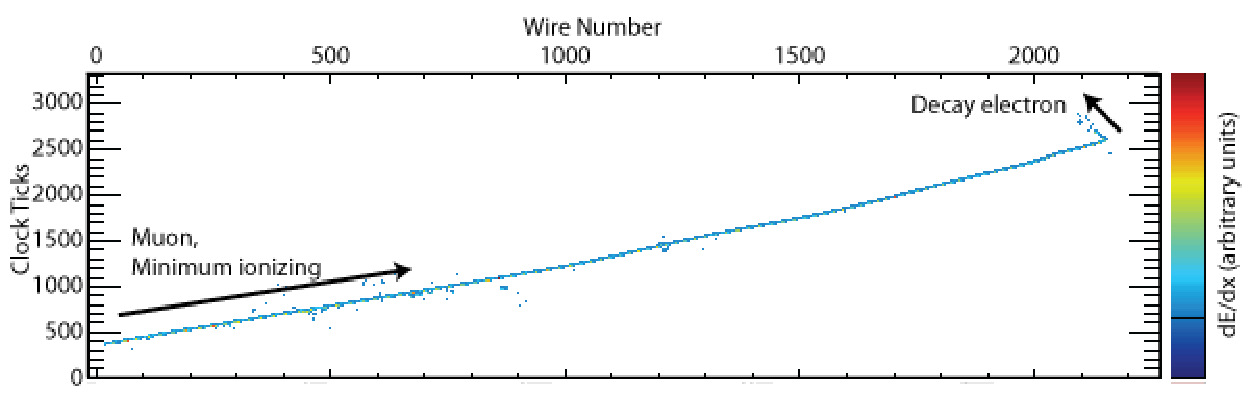
\includegraphics[width=\textwidth]{numuCC_annotated.pdf}
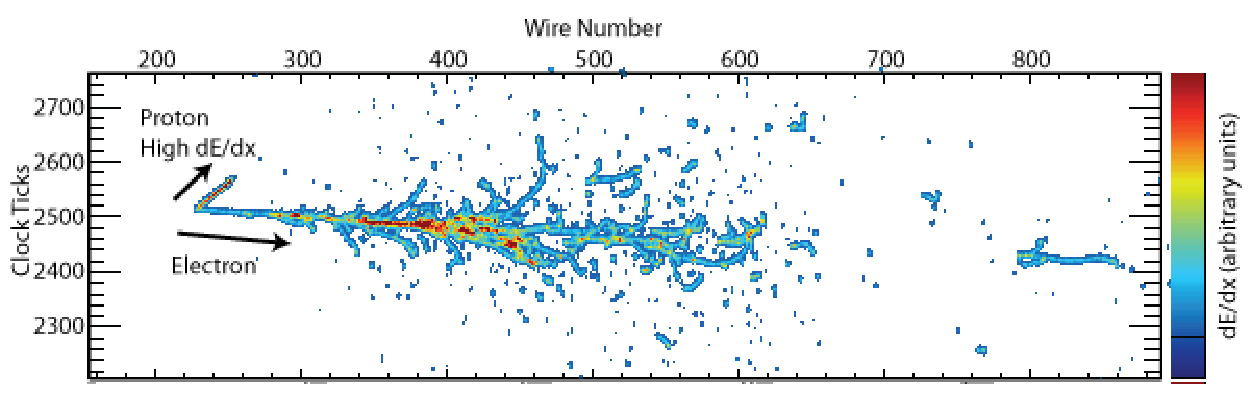
\includegraphics[width=\textwidth]{nueQE_annotated.pdf}
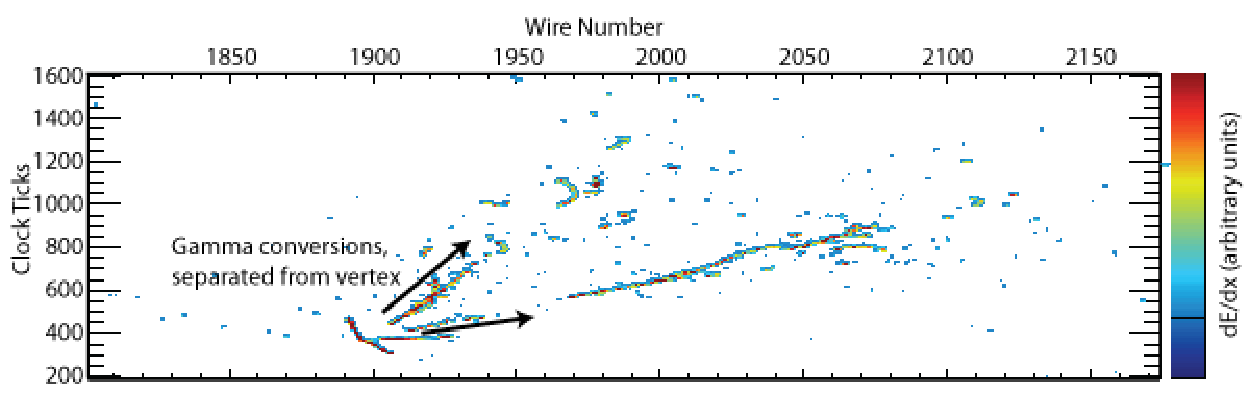
\includegraphics[width=\textwidth]{nc_pi0sep_annotated.pdf}
\end{cdrfigure}

\subsection{Far Detector Reconstruction}
\label{sec:detectors-sc-physics-software-reconstruction-fd}

The reconstruction of particle interactions in Liquid Argon TPC
detectors is an active area of research and development,
which has advanced significantly in recent years.
In particular, the data from the ICARUS~\cite{Amerio:2004ze,icarus-url,ICARUS-pizero,Antonello:2012hu} 
and ArgoNEUT experiments~\cite{Adamson:2013/02/28tla,argoneut-url,Acciarri:2013met}
have enabled the development of a variety of new reconstruction techniques,
forming the basis for precision neutrino physics measurements.
With the advancement of both single-phase and dual-phase technologies,
and expansion of the experimental program to include MicroBooNE~\cite{Chen:2007ae,microboone-url},
the 35-ton prototype and the CERN test experiments,
the reconstruction tools have continued to grow in both volume and sophistication,
supported by powerful software frameworks such as LArSoft and Qscan.

%Probably need to say around here that DUNE will require reconstruction of
%supernova bursts, atmospheric neutrinos and proton decay, not just beam neutrinos

A fully automated chain of event reconstruction algorithms
is being developed for the DUNE Far Detector.
The block diagram in figure~\ref{fig:fdrecoblockdiag} illustrates 
the components of this reconstruction chain.
The first stage of reconstruction involves the processing of the
noisy ADC wire signals, and the creation of 2D `hits'. 
These hits provide the input for a series of pattern recognition algorithms,
which form 2D and 3D clusters, representing individual particle tracks and showers.
A set of high-level algorithms are then used to reconstruct the 
3D vertex and trajectory of each particle, identify the type of particle,
and determine the four-momentum.
While each stage of the reconstruction chain has been implemented,
the algorithms are not yet fully optimised and are subject to
continuous improvement.

\begin{cdrfigure}[Far detector reconstruction block diagram]{fdrecoblockdiag}
{Block diagram showing the far detector reconstruction chain}
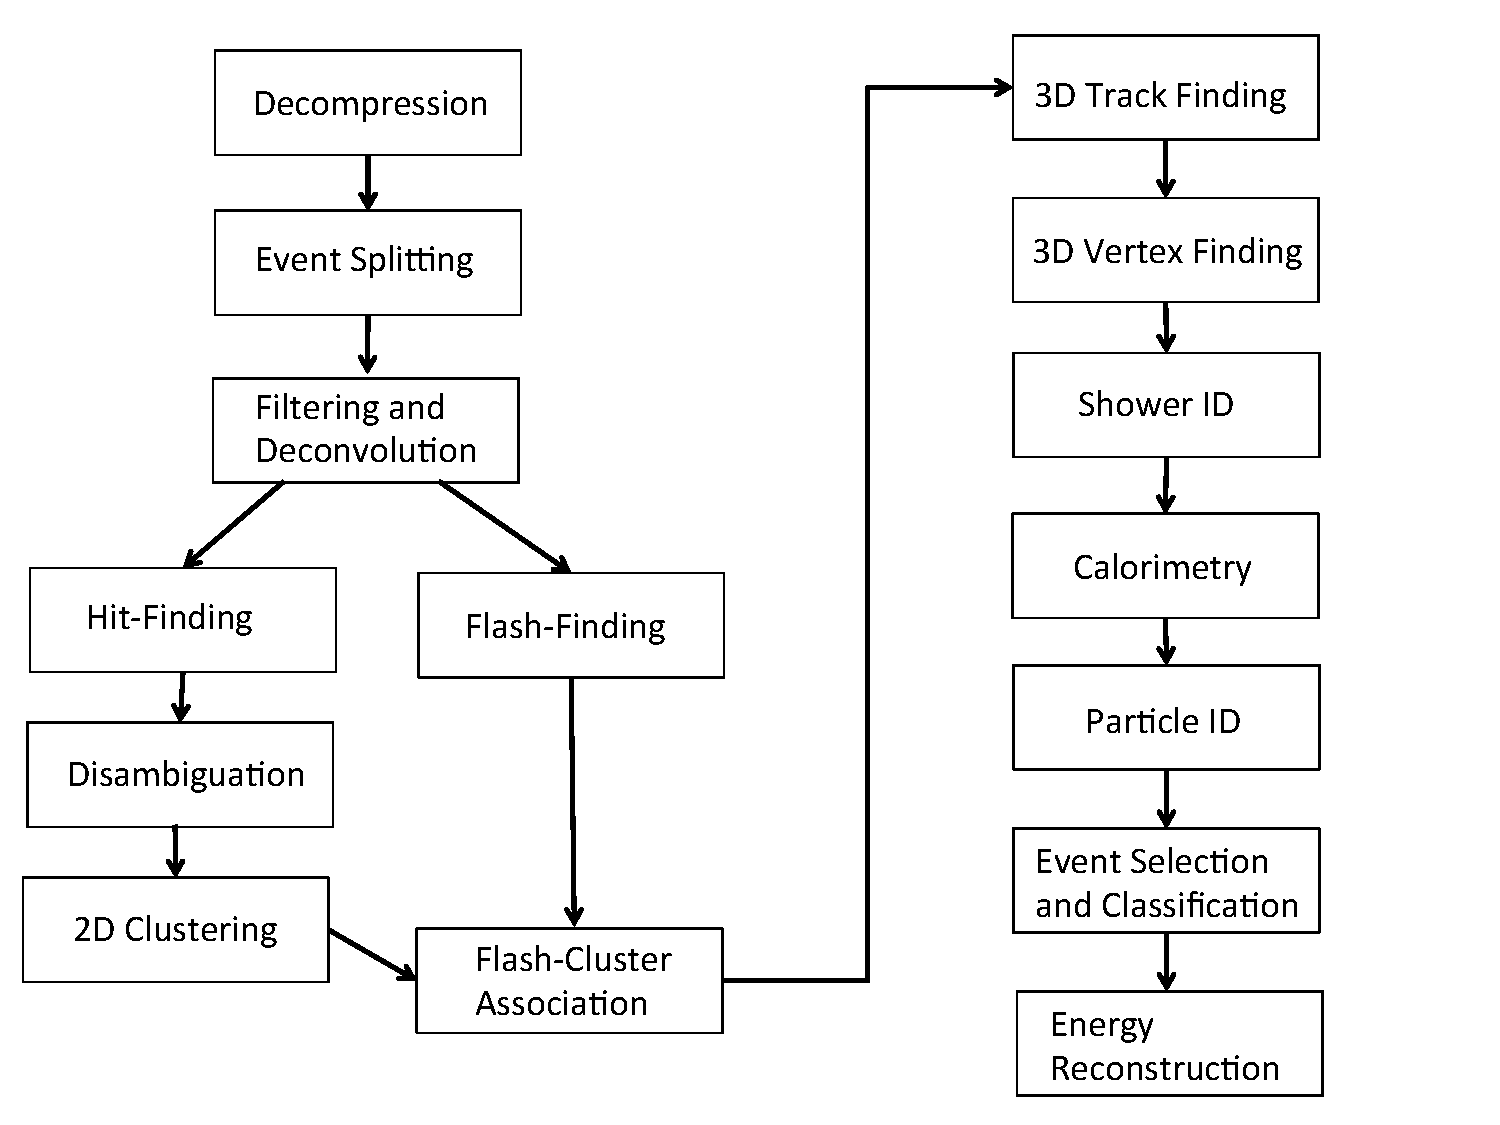
\includegraphics[width=0.8\textwidth]{fdrecoflowchart.pdf}
\end{cdrfigure}


\begin{cdrfigure}[Dual-phase LArTPC reconstructed events for data and MC]{lbnoeventsdisplay}
{
%Badertscher:2012dq
Dual-phase LArTPC reconstructed events for data and MC.
Top: Cosmic ray event displays for an hadronic shower candidate.
Bottom: Reconstructed hits for a MC simulation of a 5 GeV $\nu_{\mu}$ interaction.
The secondary particles produced in the two interactions are distinguished with different colors based on the MC truth information (blue=muon, green=electron, red=proton, cyan=pion).
}
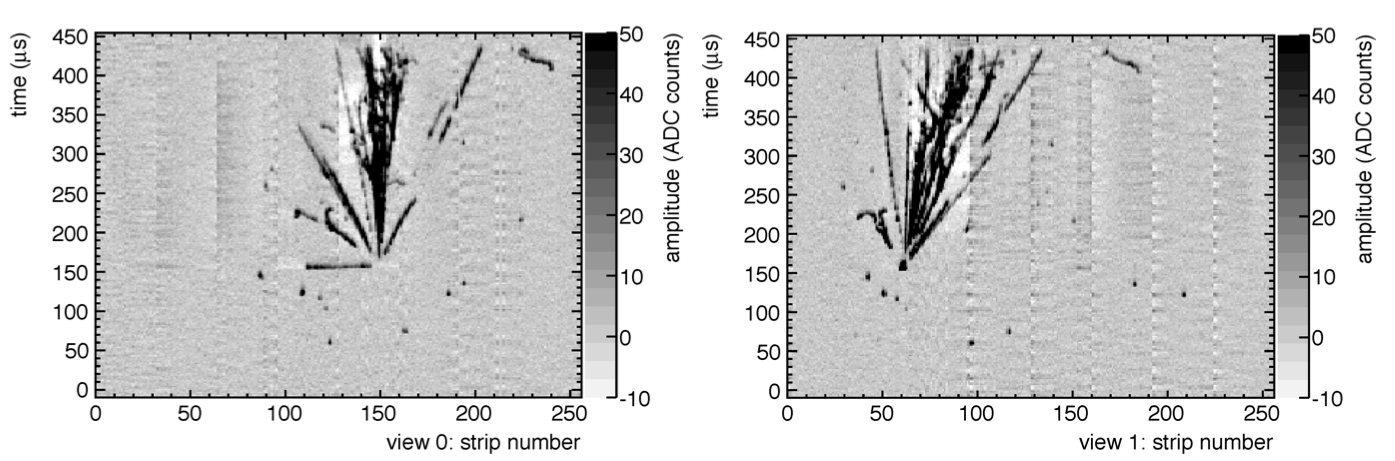
\includegraphics[width=0.99\textwidth]{LArTPC-3L-LEM-cosmics.png}
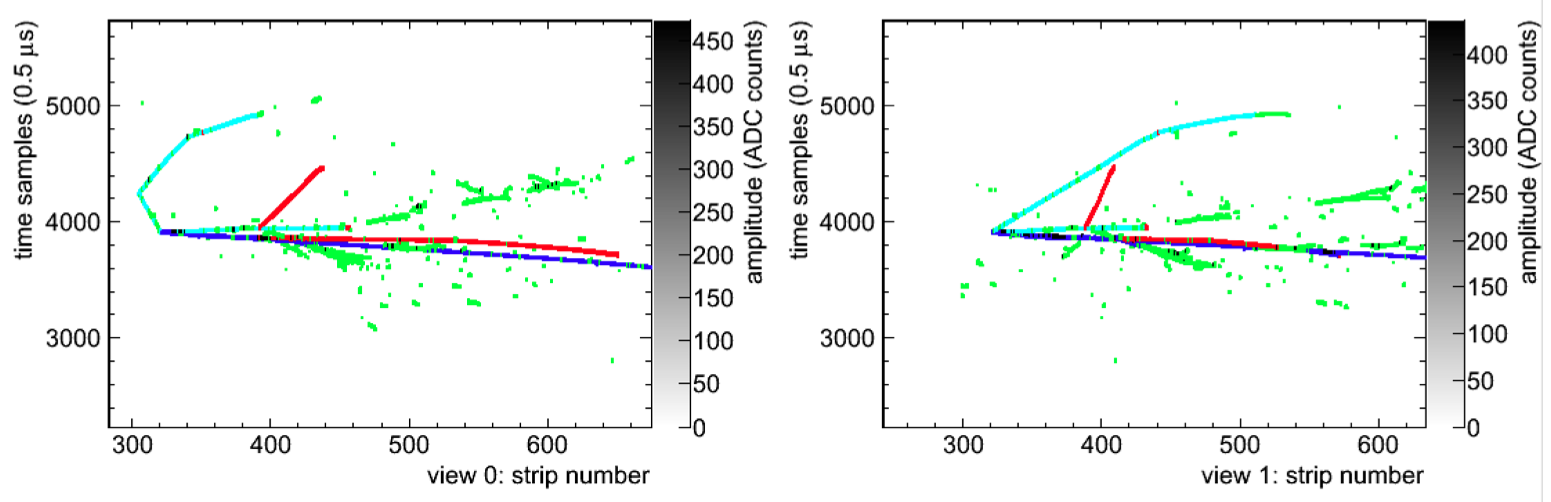
\includegraphics[width=0.99\textwidth]{LBNO-MC-nu_mu_event.png}
\end{cdrfigure}

\subsubsection{Signal Processing, Hit Finding, and Disambiguation}

Separate chains of dedicated signal-processing and hit-finding 
algorithms have been developed for the single-phase and dual-phase detectors,
as described in Sections~\ref{annex:reconstruction-signal-proc} and \ref{annex:reconstruction-single-phase-hit-find}.
The single-phase hit reconstruction proceeds by filtering noise
from the uncompressed data, and then deconvoluting the 
detector and electronics response.
The pulse-shape models used to deconvolute the response are currently
based on {\it a priori} predictions, but these will be tuned and
validated using data from the 35-ton prototype and CERN test experiment.
The current algorithms are found to perform well in ArgoNeuT analyses~\cite{Anderson:2012vc}.
After deconvolution and pedestal subtraction, pulses are identified in
the waveforms, and parametric fits are applied to extract the size and
shape of each pulse. These pulses are called hits for later processing.
At this stage, the data are still two-dimensional -- each hit provides
a wire location and a measurement of time and total charge,
but no indication of where along a wire the charge was deposited.
Hits may also overlap if they are close together in time, 
even if the charge was deposited on distant segments of the wire.

%\fixme{3L dual-phase proto hit reco}
In the dual-phase detector, the raw waveforms also undergo initial processing, 
ensuring effective noise reduction and subtraction of the baseline.
Hits, defined as signals that are discriminated from the noise, are then identified and reconstructed.
The hit-finding algorithms extract multiple hit information by fitting the waveform function of the signal.
The main parameters determined by the fits are the hit time and the integrated hit charge.
The full hit-reconstruction procedure has been successfully tested during several phases 
of R$\&$D and prototyping on small-scale double phase LAr-LEM-TPC setups \cite{Badertscher:2008rf,Badertscher:2012dq}.
Figure~\ref{fig:lbnoeventdisplay} shows example event displays of the reconstructed hits 
in both real and simulated data. 

The wrapping of induction-plane wires in the single-phase APA design
introduces an additional discrete ambiguity in the data by connecting multiple wire
segments to each DAQ channel. A ``disambiguation'' algorithm,
described in Section~\ref{annex:reco-disambiguation}, is used to break the
ambiguity and determine which wire segment generated the charge on each hit.
The algorithm forms associations between the collection view and induction views,
identifying ``triplets'' of hits that have intersecting wire segments
and consistent arrival times. In most events, the majority of hits are
associated with a single wire segment, and can be trivially disambiguated.
The remaining hits are then disambiguated by clustering them with trivially disambiguated hits.
The performance of the disambiguation algorithm is discussed in the Section~\cite{annex:disambiguation}.





\subsubsection{Optical Detector Signal Reconstruction}

Optical detector signals are processed in similar ways to those on the TPC wires.
Noise is filtered out, and hits are identified as pulses above the pedestal.
Hits are grouped together into clusters, called ``flashes'', for subsequent
association with clusters in the TPC.  Each flash has a total integrated charge and a position
estimate.


\subsubsection{TPC Pattern Recognition}

After the hit-finding and disambiguation stages have completed, a series of 
pattern recognition algorithms are applied to the 2D hits in order to identify 
the 3D tracks and showers produced by individual final-state particles in an event.
The reconstruction of 3D particles can be accomplished either by forming 2D clusters
and associating them between views, or by first associating 2D hits between views
and then clustering the resulting 3D hits. 
The clustering of hits in Liquid Argon TPC detectors is a challenging task
due to the variety and complexity of event topologies.
However, several automated 2D and 3D pattern recognition algorithms have been 
implemented using a range of techniques.

One promising suite of reconstruction tools is the 
PANDORA software development kit~\cite{Marshall:2013bda,Marshall:2012hh}
which provides fully-automated pattern recognition for both single-phase 
and dual-phase technologies. 
PANDORA implements a highly modular approach to pattern recognition,
in which events are reconstructed using a large chain of algorithms. 
A series of 2D pattern recognition algorithms are first applied,
which cluster together nearby hits based on event topology.
The resulting 2D clusters are then associated between views
and built into 3D tracks and showers, modifying the 2D clustering 
as needed to improve the 3D consistency of the event. 
Vertex-finding algorithms are also applied,
and neutrino events are reconstructed by associating the 
3D particles to the primary interaction vertex.

Figure~\ref{fig:pandoraefficiency} shows the current efficiency for reconstructing
the leading final-state lepton as a function of its momentum
for 5\,GeV $\nu_{e}$ and $\nu_{\mu}$ charged-current interactions
simulated in the MicroBooNE detector.
In both samples, the reconstruction efficiency increases rapidly with momentum,
rising above 90\% at 500\,MeV and reaching approximately 100\% at 2\,GeV.
Figure~\ref{fig:recoannexpandoravertexresolution} shows the spatial resolution for
reconstructing the primary interaction vertex in these 5\,GeV event samples,
projected onto the $x$, $y$ and $z$ axes. An estimate of the overall vertex 
resolution is obtained by taking the 68\% quantile of 3D vertex residuals, 
which yields 2.2\,cm (2.5\,cm) for $\nu_{\mu}$ CC ($\nu_{e}$ CC) events.

\begin{cdrfigure}[PANDORA reconstruction efficiency]{pandoraefficiency}
{Reconstruction efficiency of Pandora pattern recognition algorithms
 for the leading final-state lepton in 5\,GeV $\nu_{\mu}$ CC (left) and
 $\nu_{e}$ CC (right) neutrino interactions, plotted as a function of
 the lepton momentum. The reconstruction performance is evaluated
 using the MicroBooNE detector geometry. }
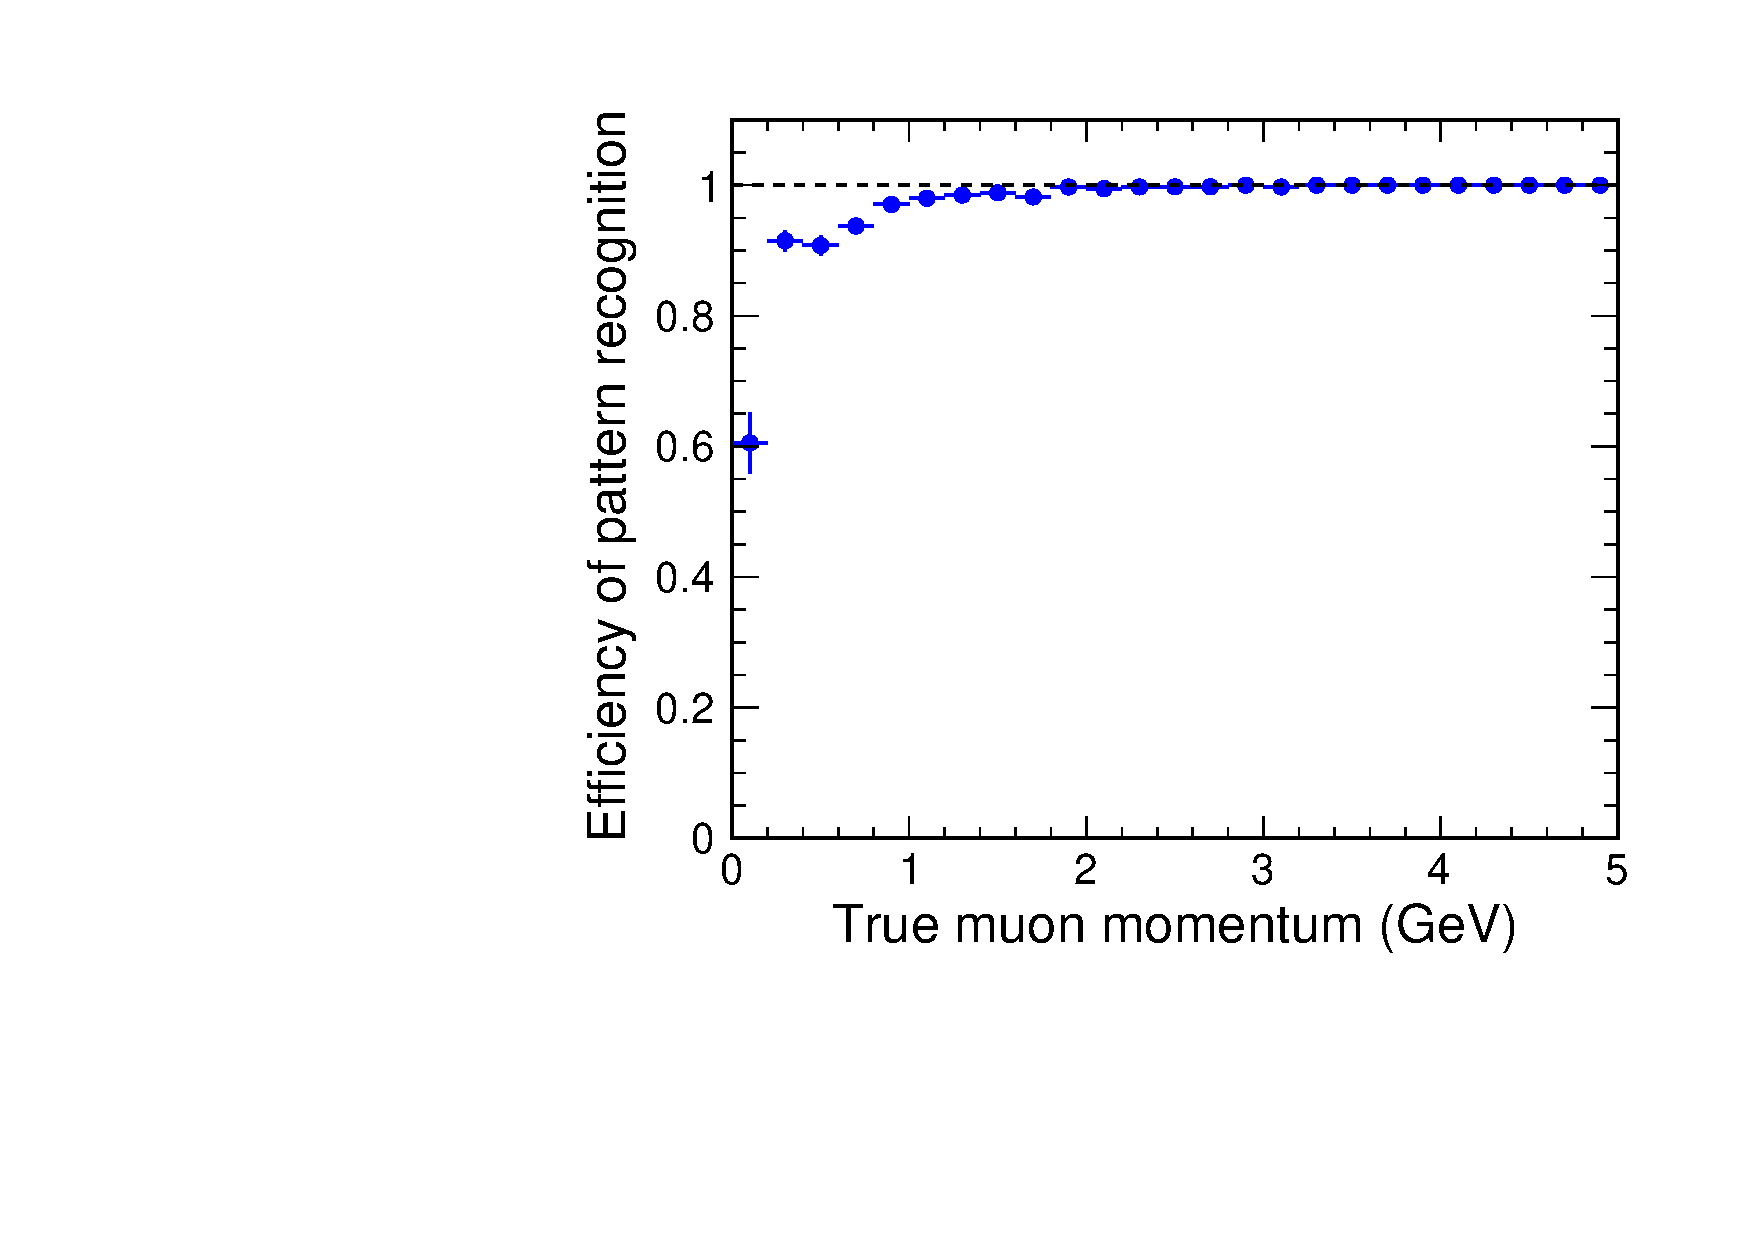
\includegraphics[width=0.49\textwidth]{pandora_uboone_efficiency_5GeV_numucc.pdf}
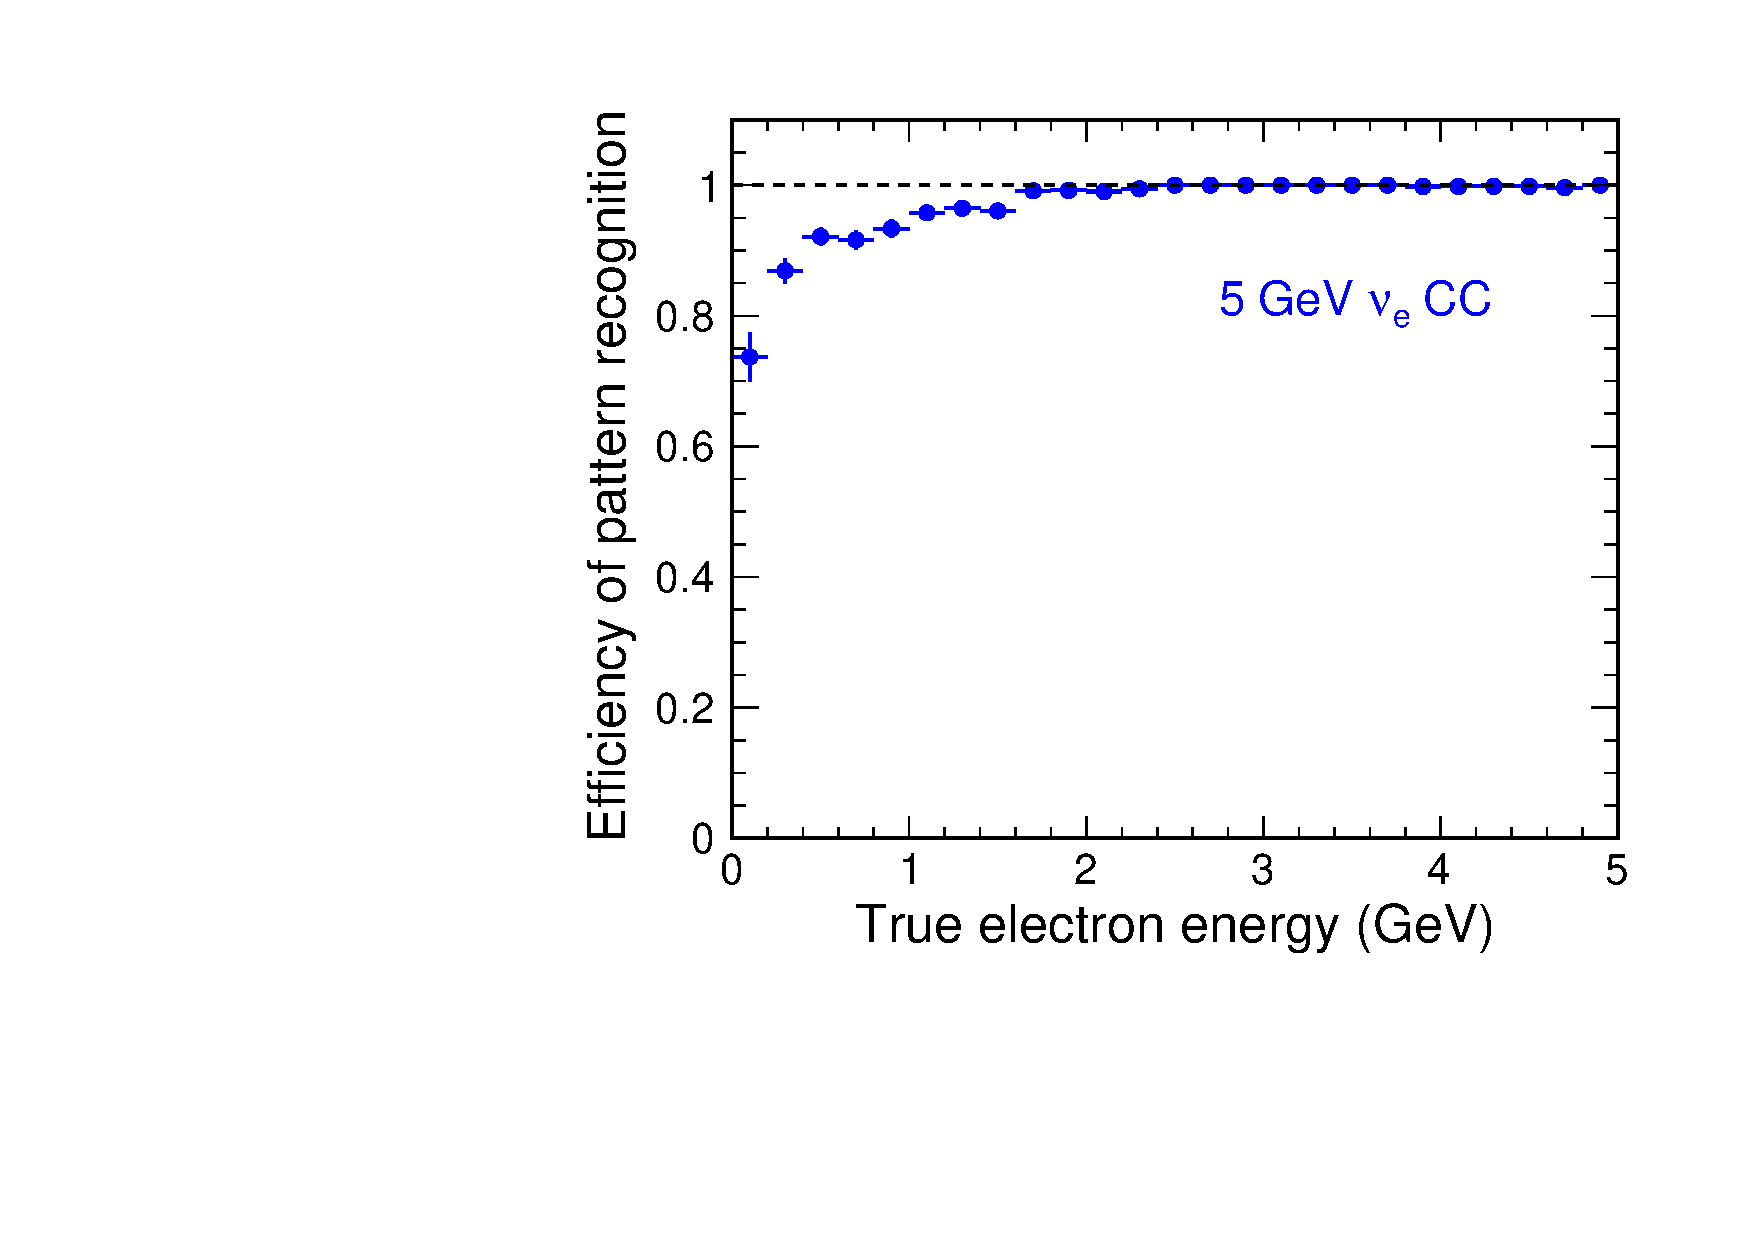
\includegraphics[width=0.49\textwidth]{pandora_uboone_efficiency_5GeV_nuecc.pdf}
\end{cdrfigure}

\begin{cdrfigure}[PANDORA vertex resolution]{recoannexpandoravertexresolution}
{Distribution of 2D residuals between reconstructed and simulated interaction
 vertex for 5\,GeV $\nu_{\mu}$ CC (left) and $\nu_{e}$ CC (right) interactions in the MicroBooNE detector.
 The $x$ axis is oriented along the drift field, the $y$ axis runs parallel 
 to the collection plane wires, and the $z$ axis points along the beam direction.}
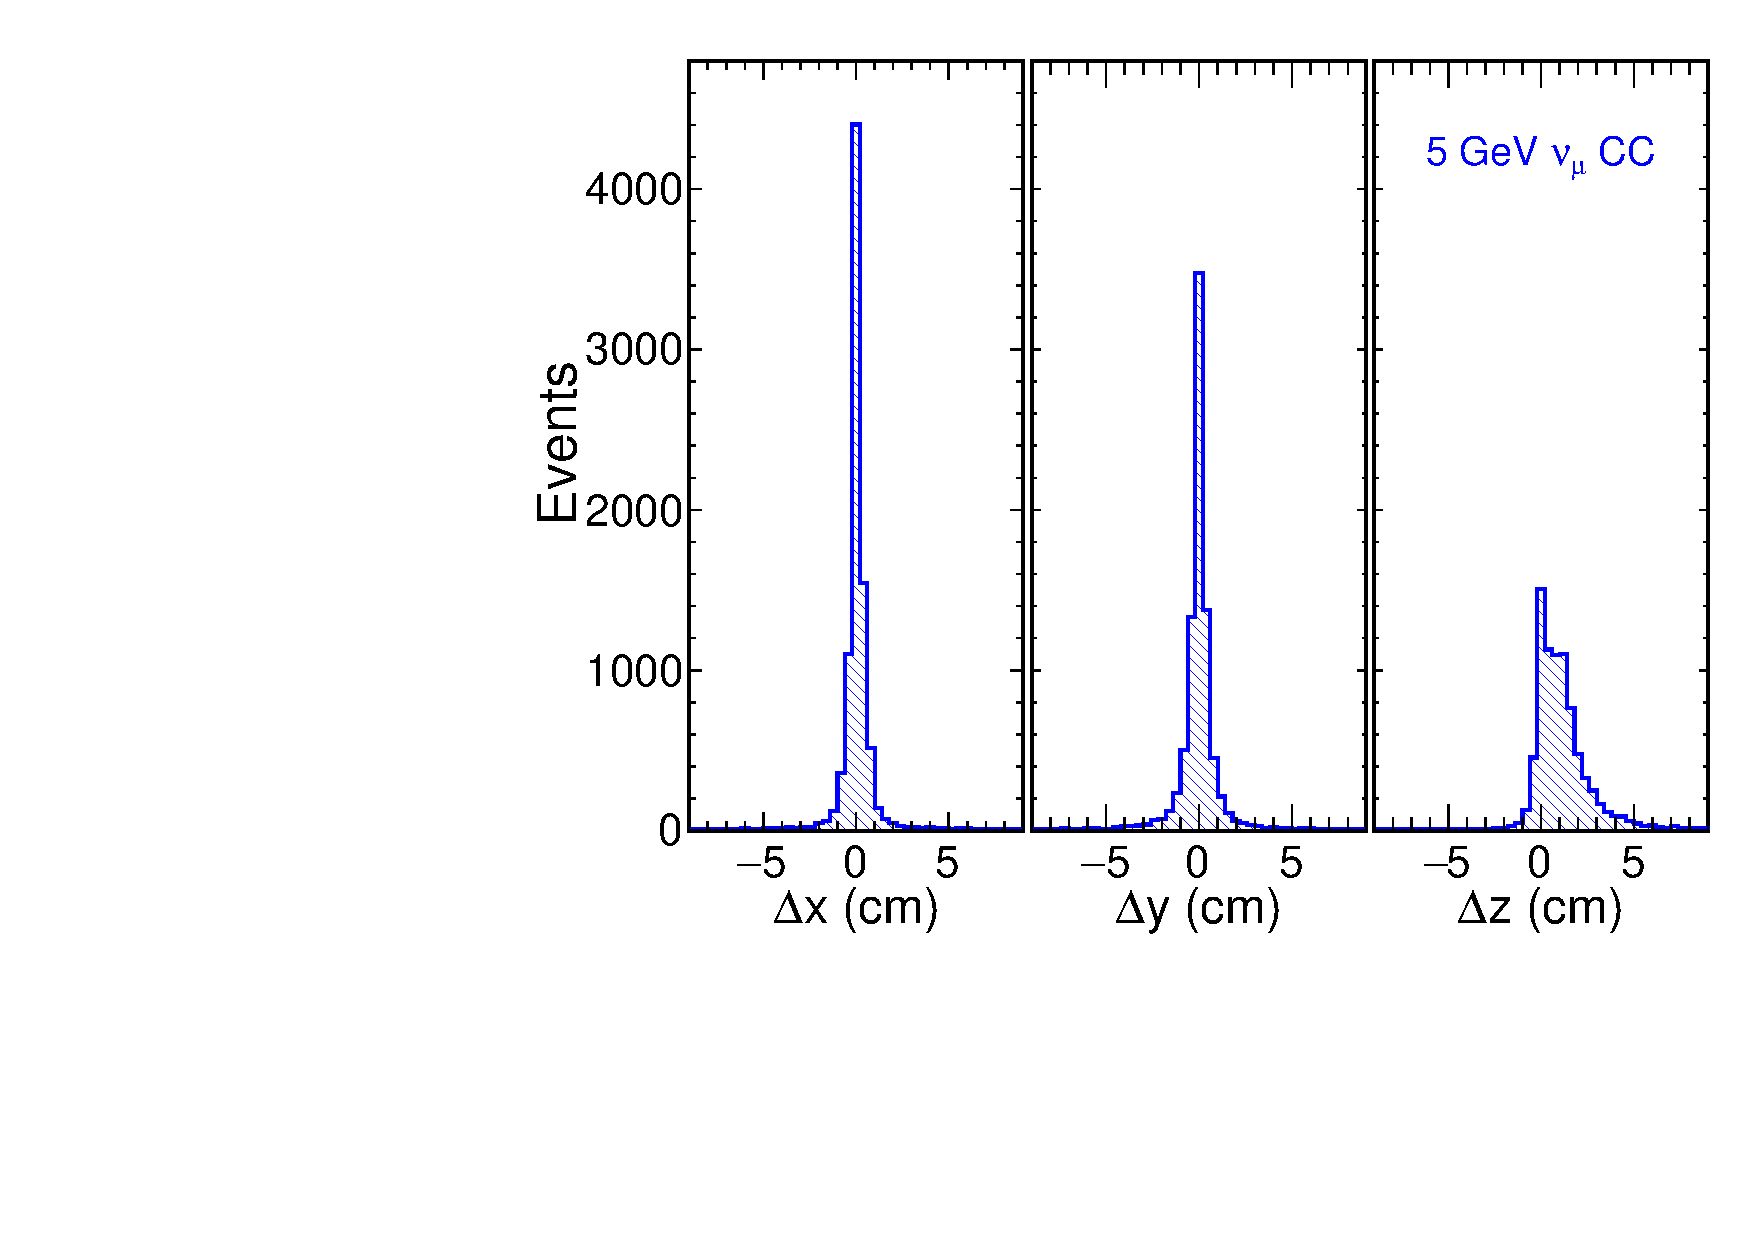
\includegraphics[width=0.49\textwidth]{pandora_uboone_vertex_resolution_numucc.pdf}
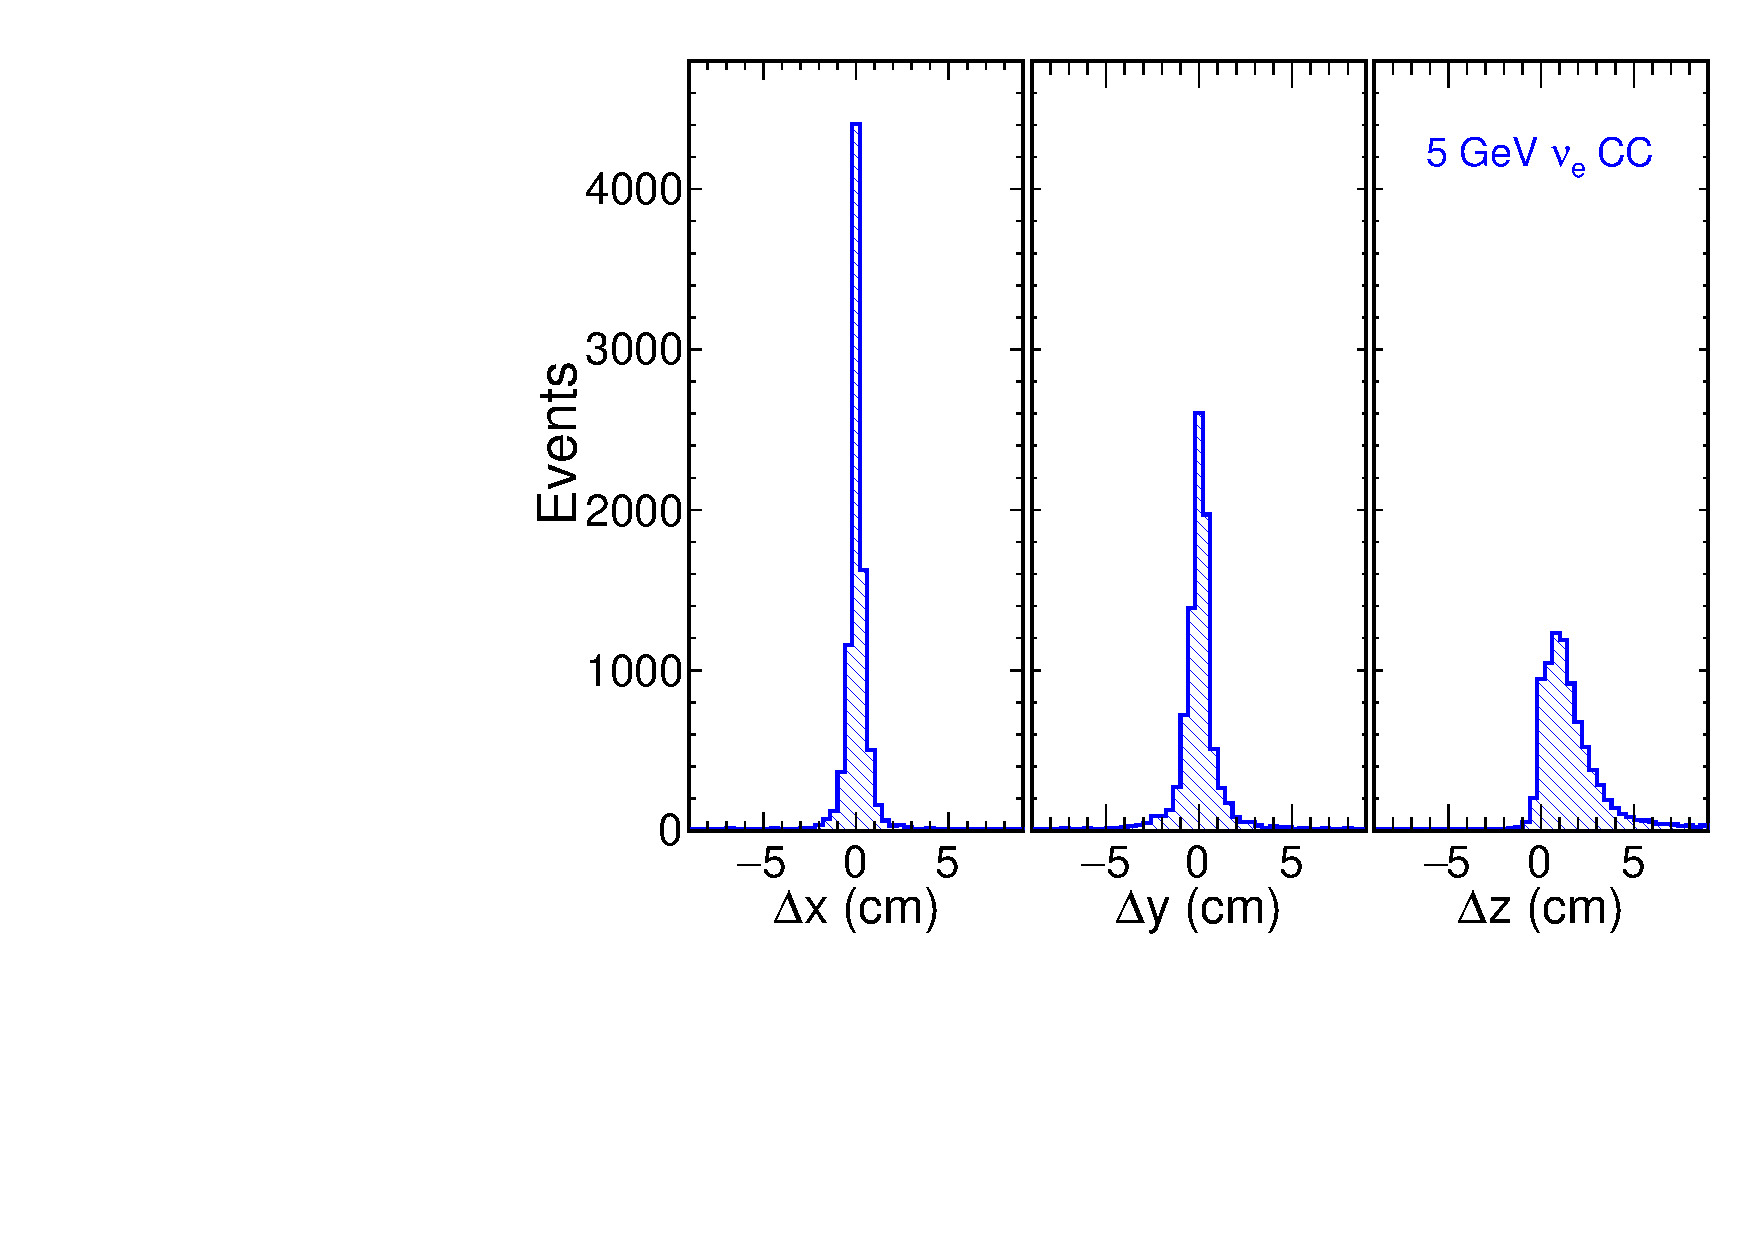
\includegraphics[width=0.49\textwidth]{pandora_uboone_vertex_resolution_nuecc.pdf}
\end{cdrfigure}

\subsubsection{Track Fitting and Shower Measurement}

%%%% TODO: Fix the ArgoNeuT reference: Can't find the words Kalman Filter 
%%%%       in any of their papers. Statement comes from MicroBooNE TDR.

After the pattern recognition stage, a series of high-level reconstruction
algorithms are applied to the 2D and 3D clusters,
which fit the trajectories of particle tracks and measure the
spatial and calorimetric properties of electromagnetic and hadronic showers.
A range of different high-level techniques have been demonstrated 
for use in Liquid Argon TPC detectors using both real and simulated data.

The Kalman filter technique~\cite{kalman} is well-established in high energy physics,
and has been applied to 3D track reconstruction by both ICARUS~\cite{Ankowski:2006ts} and ArgoNEUT~\cite{REF}.
The technique incorporates the effects of multiple Coulomb scattering,
enabling a scattering-based measurement of the track momentum,
which is shown by ICARUS to have a resolution as good as $\Delta p/p \approx 10\%$ 
for the most favourable track lengths~\cite{Ankowski:2006ts}.
The data from ICARUS have also been used to develop a precise
track reconstruction algorithm, which builds a 3D trajectory for each track by simultaneously
optimising its 2D projections to match the observed data~\cite{Antonello:2012hu}.
Another promising track reconstruction technique, based on the local principal curve algorithm,
has been implemented in conjunction with the development of the 
dual-phase detector concept, and is shown to provide 
a precise reconstruction of two-body final states~\cite{Back:2013cva,LAGUNA-LBNO-deliv}. 

A full 3D reconstruction of electromagnetic showers is currently in development.
In the present scheme, the first stage is an examination of clusters 
in terms of their 2D parameters, and a selection of shower-like clusters 
for further analysis. The 3D start position, principal axis,
and shower shape variables are then reconstructed by matching up 2D hits between views.
These 3D parameters, combined with calorimetric information, enable a measurement
of the total shower energy, as well discrimination between electrons
and converted photons based on the ionization energy in the initial part of
the shower. The kinematic reconstruction of final-state neutral pions from their
$\pi^{0} \rightarrow \gamma\gamma$ decays can be performed by 
combining together associated pairs of photons.


\subsubsection{Calorimetry and Particle Identification}

The measurement of the ionization density $dE/dx$ is important
for particle identification and energy measurement.
In order to reconstruct this information, the measured charge on each hit 
is first obtained from fits to the pulse shapes.
The charge loss due to the finite electron lifetime is corrected
based on the time of the event, and the path length corresponding
to each hit is calculated based on the event trajectory.
The effects of recombination, known as ``charge quenching''
are corrected using a modified Box model~\cite{Thomas:1987zz} 
or Birks' Law`\cite{Birks:1964zz}.
The identity of a particle track which ranges out in the active detector volume
may be ascertained by analysing the ionization density $dE/dx$ as a function of 
the range from the end of the track, and comparing with the predictions
for different particle species. Various analysis techniques have been developed
for this purpose, as described in Section~\ref{annex:reco-pid}.
 
%\fixme{Do we have any calorimetry plots?}

\subsubsection{Neutrino Event Reconstruction and Classification}

Once all the final-state particles in an event have been reconstructed individually, 
the combined information is used to reconstruct and classify the overall event.
The identification of neutrino event types is based on a 
multivariate analysis~\cite{Back:2013cva,WA105_TDR,LAGUNA-LBNO-deliv,LAGUNA-LBNO-EOI},
which constructs a number of characteristic topological and calorimetric variables,
based on the reconstructed final-state particles. In the present scheme,
a Boosted Decision Tree algorithm is used to calculate signal and background likelihoods 
for particular event hypotheses. The current performance has been evaluated using fully reconstructed
$\nu_{e}$ and $\nu_{\mu}$ charged-current interactions with two-body final states,
simulated in the dual-phase Far Detector~\cite{LAGUNA-LBNO-deliv}. 
The correct hypothesis is chosen for 92\% (79\%) of $\nu_{\mu}$ ($\nu_{e}$) quasi-elastic interactions 
with a lepton and proton in the final state, and 79\% (71\%) of $\nu_{\mu}$ ($\nu_{e}$) 
resonance interactions with a lepton and charged pion in the final state.
For selected events, the neutrino energy is estimated kinematically for quasi-elastic interactions
using a two-body approximation, or otherwise a calorimetric energy measurement is applied.
The calorimetric reconstruction takes into account the quenching factors of the different particles, 
assuming that all hits not associated with the primary lepton are due to hadronic activity.
Figure~\ref{fig:recoenergynue} shows the resulting energy reconstruction for $\nu_e$ CCQE and CC1$\pi^{+}$ events.

\begin{cdrfigure}[Reconstruction of electron neutrino energy]{recoenergynue}
{Performance of neutrino energy measurement, evaluated using the dual-phase far detector simulation. 
Distributions of reconstructed versus true neutrino are shown for $\nu_{e}$ CCQE events (left),
assuming two-body kinematics, and $\nu_{e}$  CC1$\pi^{+}$ events (right),
using a calorimetric energy estimation.}
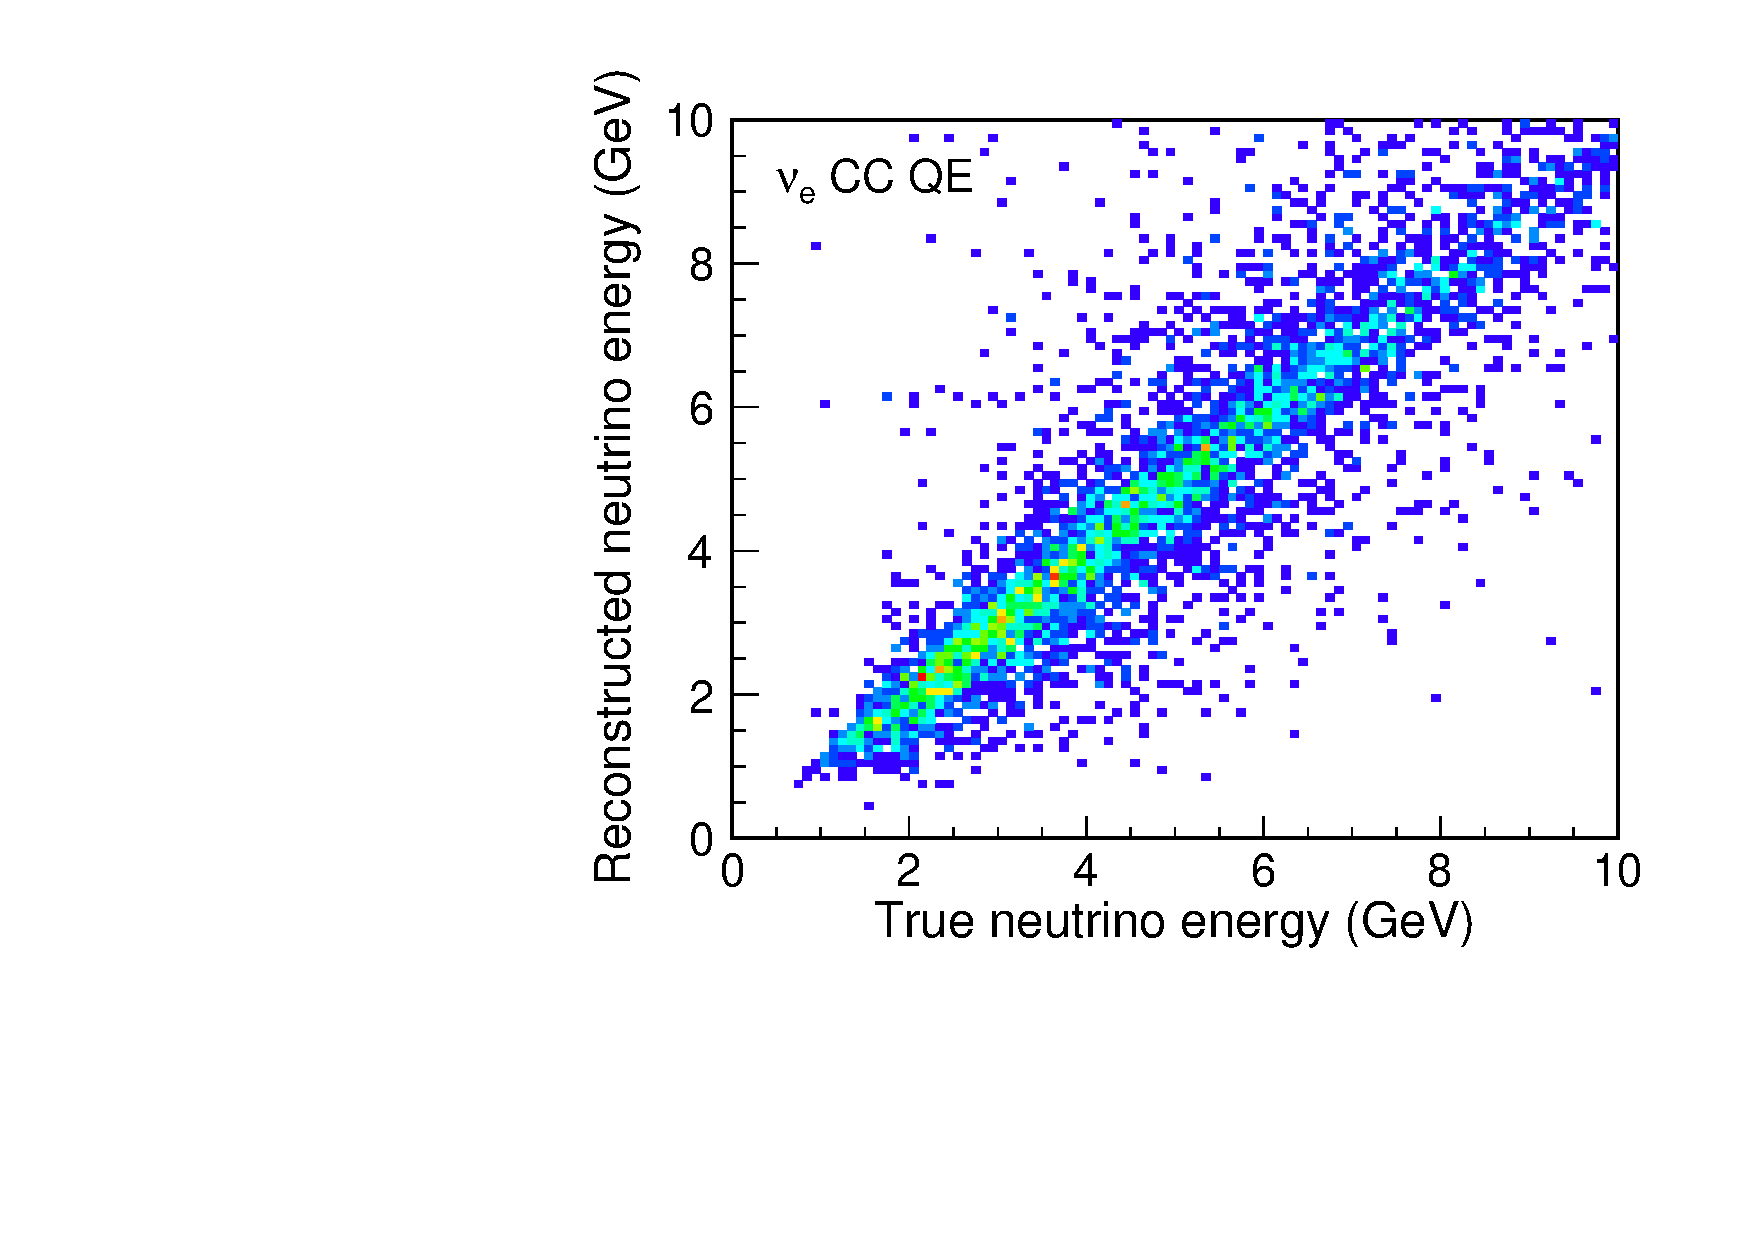
\includegraphics[width=0.49\textwidth]{laguna_lbno_recoenergy_nue_ccqe.pdf}
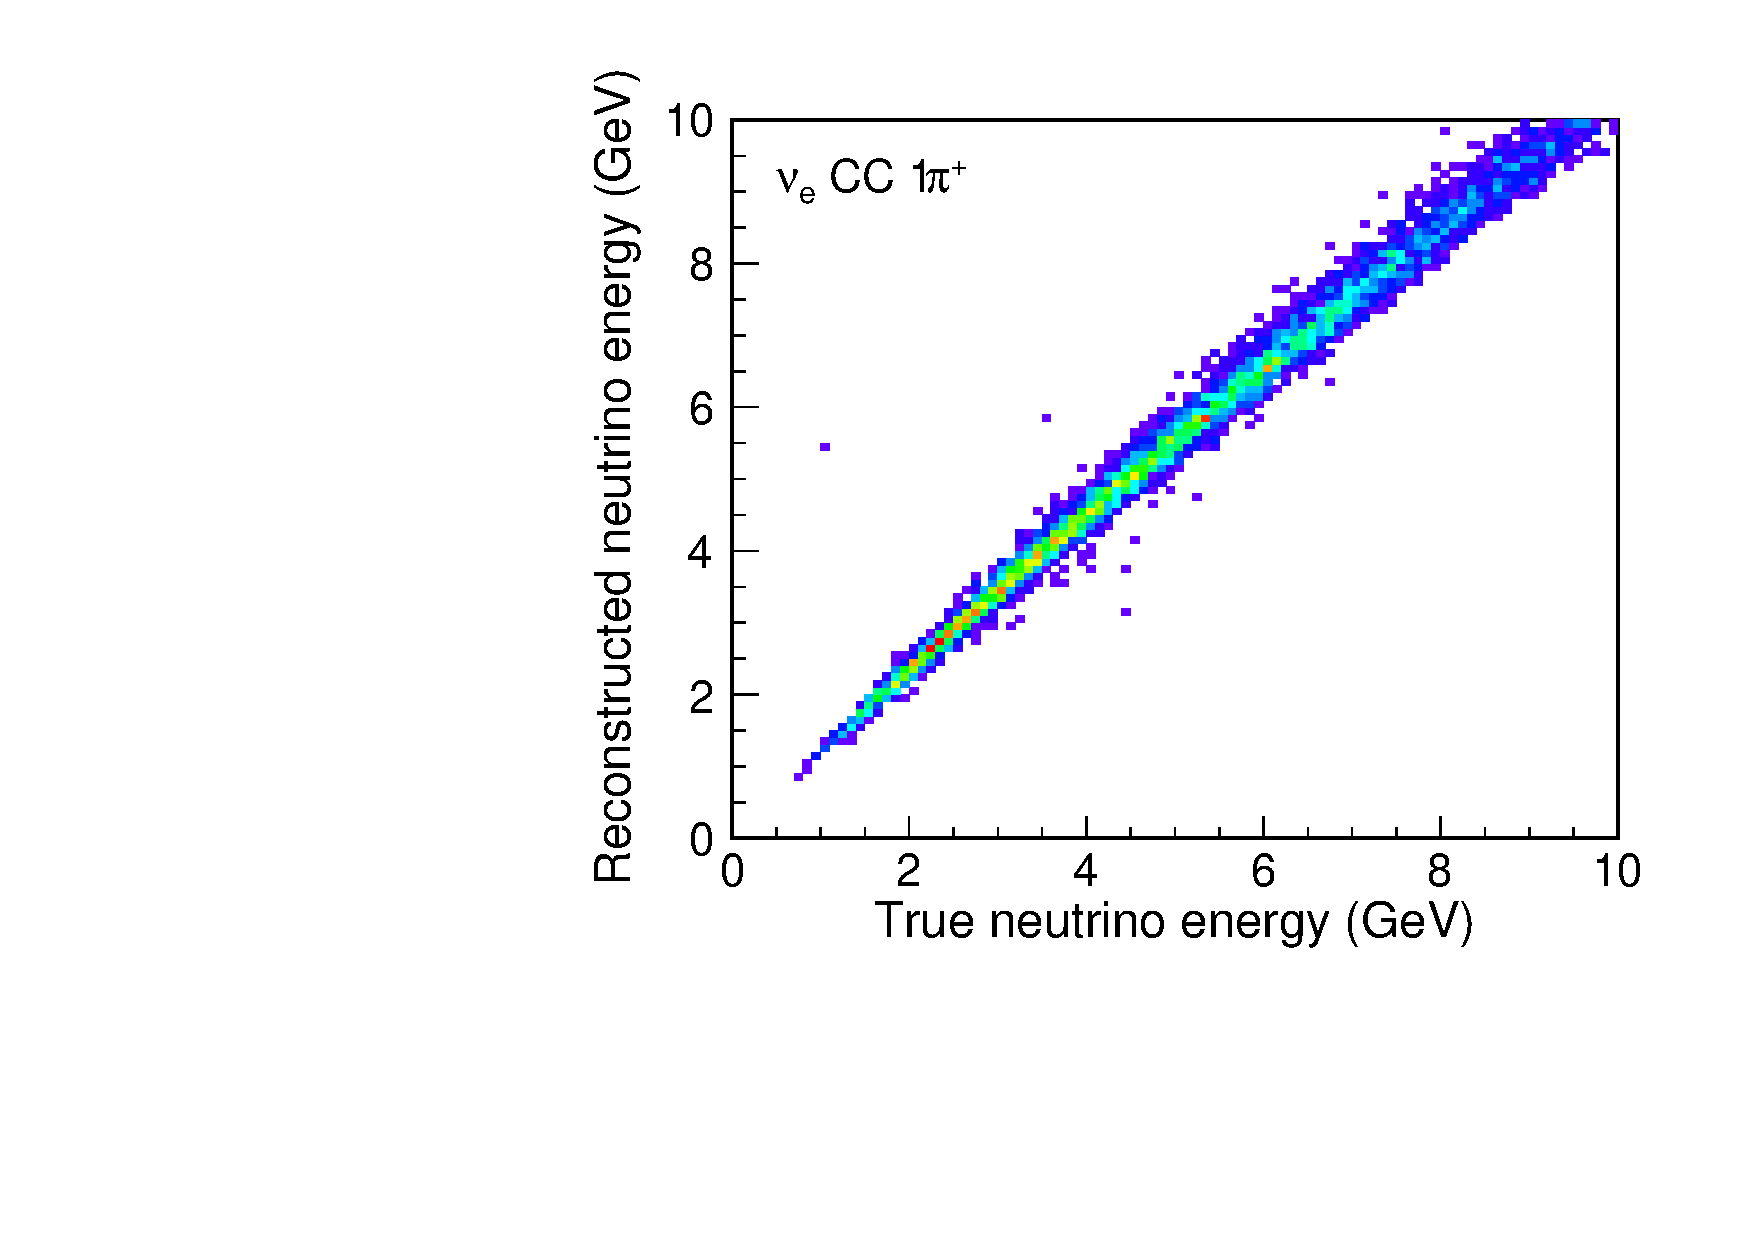
\includegraphics[width=0.49\textwidth]{laguna_lbno_recoenergy_nue_ccres.pdf}
\end{cdrfigure}

%%%% Do we need a summary?

